% !TeX spellcheck = en_US
\documentclass[slidestop,usenames,dvipsnames]{beamer}
\usepackage[utf8]{inputenc}
\usepackage{fancyvrb}
\usepackage[absolute,overlay]{textpos}
\usepackage{comment}
\usepackage{newunicodechar}
\usepackage{graphicx}
\newunicodechar{💃}{
\includegraphics{dancer}}

\title{Idman 2 -- Electric Boogaloo}
\subtitle{💃💃💃\ Still Doing the Identity Management Dance 💃💃💃}
\author{Marco Brack \and Carsten Hartenfels \and Michael Monschau}
%\date{2016-05-31}

\beamertemplatenavigationsymbolsempty
\usetheme{Boadilla}
\usecolortheme{whale}
\setbeamertemplate{itemize items}[default]
\setbeamertemplate{enumerate items}[default]
\defbeamertemplate*{footline}{my infolines theme} {
    \leavevmode
    \hbox{
    \begin{beamercolorbox}[wd=.333333\paperwidth,ht=2.25ex,dp=1ex,center]{author in head/foot}
        \usebeamerfont{author in head/foot}Brack, Hartenfels, Monschau
    \end{beamercolorbox}
    \begin{beamercolorbox}[wd=.333333\paperwidth,ht=2.25ex,dp=1ex,center]{title in head/foot}
        \usebeamerfont{title in head/foot}Idman 2 -- Electric Boogaloo
    \end{beamercolorbox}
    \begin{beamercolorbox}[wd=.309\paperwidth,ht=2.25ex,dp=1ex,center]{date in head/foot}
        \usebeamerfont{date in head/foot}\insertshortdate{}\hspace*{2em}
        \insertframenumber{} / \inserttotalframenumber\hspace*{2ex}
    \end{beamercolorbox}}
    \vskip0pt
}

\newcounter{FrameCounter}
\newcommand{\nextframe}[0]{\stepcounter{FrameCounter}}
\newcommand{\framecount}[1]{\frametitle{\arabic{FrameCounter}. {#1}}}
\newcommand{\fitem}{\pause\vfill\item}
\newcommand{\gitem}{\vfill\item}
\newcommand{\fimage}[2]{\pause\vfill\begin{center}\includegraphics[width={#2}]{#1}\end{center}}

\begin{document}

\begin{frame}
    \titlepage
\end{frame}


%%%%%%%%%%%%%%%%%%%%%%%%%%%%%%%%%%%%%%%%%%%%%%%%%


\begin{frame}
    \frametitle{Content}
    \begin{itemize}
       \gitem More Results
       \gitem Ground Truth
       \gitem Some Graphs
       \gitem Usage
    \end{itemize}
    \vfill
\end{frame}


\begin{frame}
  \frametitle{Algorithm Performance: Bird ($t=0.8$)}
  Example Repo: \texttt{django-oscar}
  \begin{itemize}
    \gitem Wrongly Merged: \textbf{50}
    \gitem Not Merged: \textbf{0}
    \gitem Correctly Merged: \textbf{155}
  \end{itemize}
  \begin{itemize}
    \gitem recall: \textbf{1} (Bird merged all of the identities that had to be merged)
    \gitem precision: \textbf{0.756} (Not all merged identities should have been merged)
    \gitem fmeasure: \textbf{0.861}
  \end{itemize}
  \vfill
\end{frame}


\begin{frame}
  \frametitle{Algorithm Performance: Bird ($t=0.9$)}
  Example Repo: \texttt{django-oscar}
  \begin{itemize}
    \gitem Wrongly Merged: \textbf{43} (Less)
    \gitem Not Merged: \textbf{0}
    \gitem Correctly Merged: \textbf{162} (More)
  \end{itemize}
  \begin{itemize}
    \gitem recall: \textbf{1} (Bird merged all of the identities that had to be merged)
    \gitem precision: \textbf{0.79} (Not all merged identities should have been merged)
    \gitem fmeasure: \textbf{0.882} (Better)
  \end{itemize}
  \vfill
\end{frame}


\begin{frame}
  \frametitle{Algorithm Performance: Occurrence}
  Example Repo: \texttt{django-oscar}
  \begin{itemize}
    \gitem Wrongly Merged: \textbf{0} (Much less)
    \gitem Not Merged: \textbf{3} (Little more)
    \gitem Correctly Merged: \textbf{202} (Much more)
  \end{itemize}
  \begin{itemize}
    \gitem recall: \textbf{1} (Merged all of the identities that had to be merged)
    \gitem precision: \textbf{0.985} (Only few merged identities should not have been merged)
    \gitem fmeasure: \textbf{0.992} (Much better)
  \end{itemize}
  \vfill
\end{frame}


\nextframe
\begin{frame}
  \frametitle{Results}
  \begin{itemize}
    \gitem Improved Fancy Algorithms
    \gitem They Get Things Wrong Though
  \end{itemize}
  \begin{table}[]
    \centering
    \caption{Resulting Identities with Different Algorithms}
    \label{tab:results}
    \begin{tabular}{|l|c|c|c|c|c|}
      \hline
      \textbf{Repo}    & \textbf{Git} & \textbf{Occurrence} & \textbf{Default} & \textbf{Similarity} & \textbf{Bird}\\\hline
      django-cms       & 564          & 457                 & 454              & 454                 & 340\\\hline
      django-oscar     & 250          & 208                 & 207              & 206                 & 177\\\hline
      django-wiki      & 81           & 69                  & 69               & 68                  & 68\\\hline
      elasticsearch    & 913          & 797                 & 794              & 794                 & 480\\\hline
      libgdx           & 517          & 421                 & 420              & 417                 & 336\\\hline
      spring-framework & 230          & 188                 & 188              & 188                 & 173\\\hline
    \end{tabular}
  \end{table}
  \vfill
\end{frame}


\begin{frame}
  \frametitle{Results: django-cms}
  \vfill
  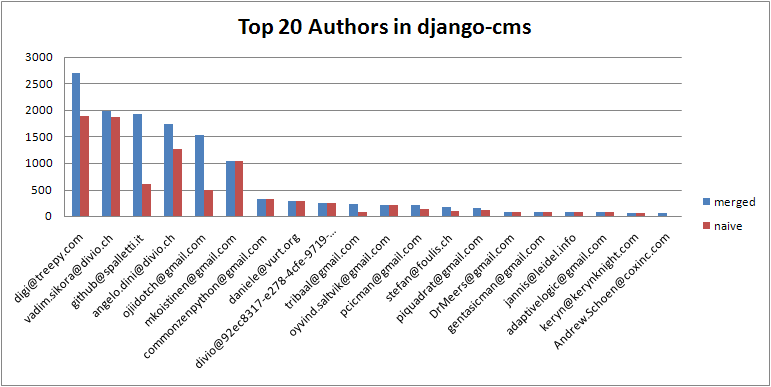
\includegraphics[width=\textwidth]{img/graph-django-cms}
  \vfill
\end{frame}

\begin{frame}
  \frametitle{Results: django-oscar}
  \vfill
  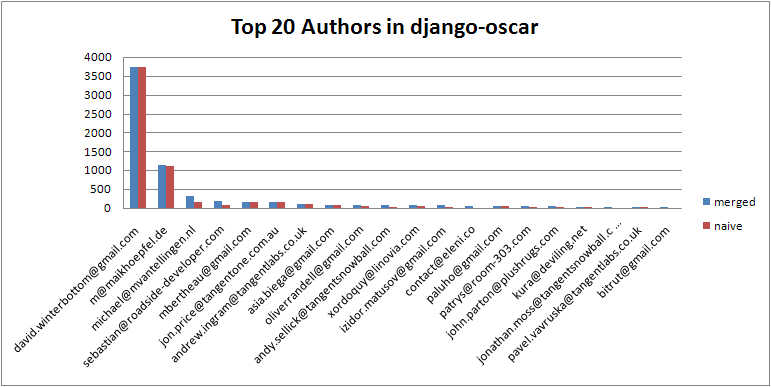
\includegraphics[width=\textwidth]{img/graph-django-oscar}
  \vfill
\end{frame}

\begin{frame}
  \frametitle{Results: django-wiki}
  \vfill
  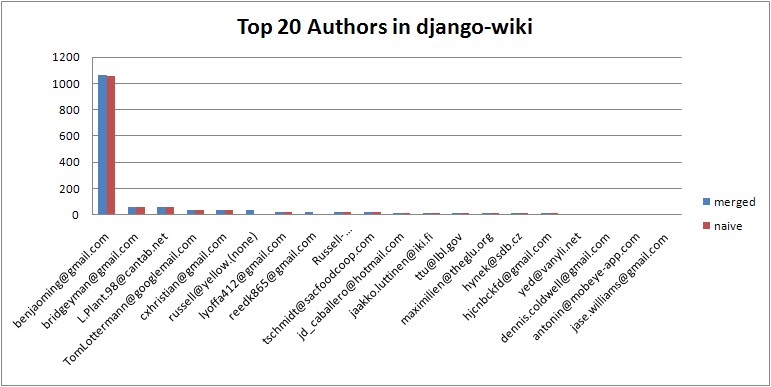
\includegraphics[width=\textwidth]{img/graph-django-wiki}
  \vfill
\end{frame}

\begin{frame}
  \frametitle{Results: elasticsearch}
  \vfill
  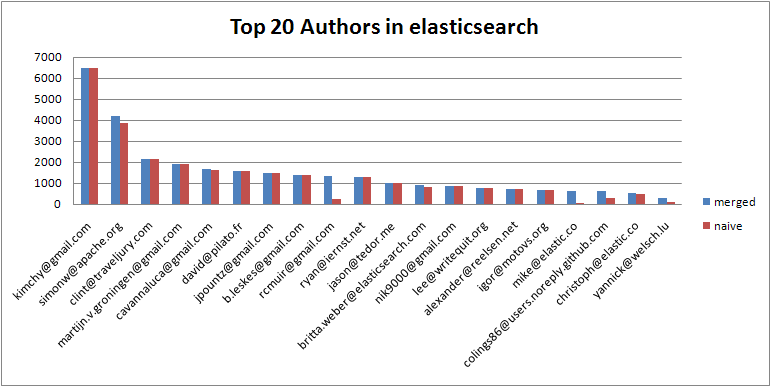
\includegraphics[width=\textwidth]{img/graph-elasticsearch}
  \vfill
\end{frame}

\begin{frame}
  \frametitle{Results: libgdx}
  \vfill
  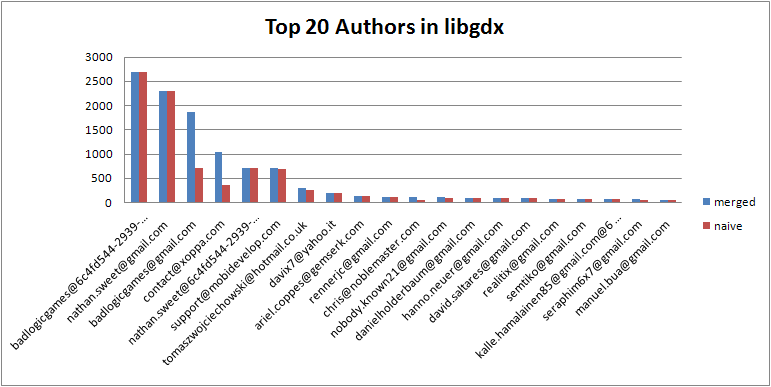
\includegraphics[width=\textwidth]{img/graph-libgdx}
  \vfill
\end{frame}

\begin{frame}
  \frametitle{Results: spring-framework}
  \vfill
  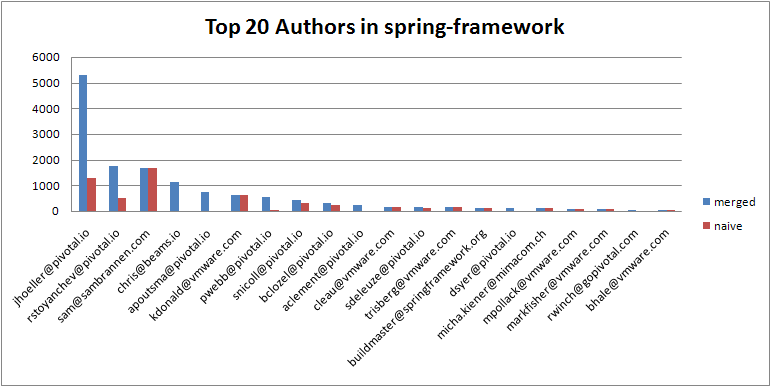
\includegraphics[width=\textwidth]{img/graph-spring-framework}
  \vfill
\end{frame}


\nextframe
\begin{frame}
    \frametitle{Usage}
    \begin{itemize}
        \gitem Clone \url{https://github.com/turbopope/idman}
        \gitem Run \texttt{idman path/to/repo}
        \gitem Get Commits With Identities
    \end{itemize}
    \vfill
\end{frame}


\begin{comment}
How many developers?
How many commiters?
What is the distribution of commit counts for committers versus authors?
The team actually addresses these questions for our ``projects of interest''.
\end{comment}


%%%%%%%%%%%%%%%%%%%%%%%%%%%%%%%%%%%%%%%%%%%%%%%%%


\nextframe
\begin{frame}
    \vfill
    \begin{center}
        {\Huge Thank You All For Listening}\\
    \end{center}
\end{frame}

\end{document}
